\section{Phase 5}
This is the fifth phase of the binary bomb. The bomb will greet you with the following lines
{\renewcommand\fcolorbox[4][]{\textcolor{black}{\strut#4}}
\begin{minted}[frame=single,framesep=10pt]{bash}
  [edusc03-052@cheetah022 bomb52]$ ./bomb input.txt
  Welcome to my fiendish little bomb. You have 6 phases with
  which to blow yourself up. Have a nice day!
  Phase 1 defused. How about the next one?
  That's number 2.  Keep going!
  Halfway there!
  So you got that one.  Try this one.
\end{minted}
}\noindent
As usual, let's enter a dummy input ``1 2'' and inspect the phase's assembly code
{\renewcommand\fcolorbox[4][]{\textcolor{cyan}{\strut#4}}
\begin{minted}[frame=single,framesep=10pt]{gas}
  0x000000000040109e <+0>:     sub    $0x18,%rsp
  0x00000000004010a2 <+4>:     lea    0x8(%rsp),%rcx
  0x00000000004010a7 <+9>:     lea    0xc(%rsp),%rdx
  0x00000000004010ac <+14>:    mov    $0x40252f,%esi
  0x00000000004010b1 <+19>:    mov    $0x0,%eax
  0x00000000004010b6 <+24>:    callq  0x400bc0 <__isoc99_sscanf@plt>
  0x00000000004010bb <+29>:    cmp    $0x1,%eax
  0x00000000004010be <+32>:    jle    0x40110a <phase_5+108>
  0x00000000004010c0 <+34>:    mov    0xc(%rsp),%eax
  0x00000000004010c4 <+38>:    and    $0xf,%eax
  0x00000000004010c7 <+41>:    mov    %eax,0xc(%rsp)
  0x00000000004010cb <+45>:    cmp    $0xf,%eax
  0x00000000004010ce <+48>:    je     0x401100 <phase_5+98>
  0x00000000004010d0 <+50>:    mov    $0x0,%ecx
  0x00000000004010d5 <+55>:    mov    $0x0,%edx
  0x00000000004010da <+60>:    add    $0x1,%edx
  0x00000000004010dd <+63>:    cltq
  0x00000000004010df <+65>:    mov    0x4023e0(,%rax,4),%eax
  0x00000000004010e6 <+72>:    add    %eax,%ecx
  0x00000000004010e8 <+74>:    cmp    $0xf,%eax
  0x00000000004010eb <+77>:    jne    0x4010da <phase_5+60>
  0x00000000004010ed <+79>:    movl   $0xf,0xc(%rsp)
  0x00000000004010f5 <+87>:    cmp    $0xf,%edx
  0x00000000004010f8 <+90>:    jne    0x401100 <phase_5+98>
  0x00000000004010fa <+92>:    cmp    %ecx,0x8(%rsp)
  0x00000000004010fe <+96>:    je     0x401105 <phase_5+103>
  0x0000000000401100 <+98>:    callq  0x401451 <explode_bomb>
  0x0000000000401105 <+103>:   add    $0x18,%rsp
  0x0000000000401109 <+107>:   retq
  0x000000000040110a <+108>:   callq  0x401451 <explode_bomb>
  0x000000000040110f <+113>:   jmp    0x4010c0 <phase_5+34>
\end{minted}
}\noindent
This function also calls \verb+sscanf+, let's see what's the pattern
{\renewcommand\fcolorbox[4][]{\textcolor{cyan}{\strut#4}}
\begin{minted}[frame=single,framesep=10pt]{bash}
  (gdb) x/s 0x40252f
  0x40252f:       "%d %d"
\end{minted}
}\noindent
So our dummy input statisfies the first constraint. Next, let's inspect the following lines
{\renewcommand\fcolorbox[4][]{\textcolor{cyan}{\strut#4}}
\begin{minted}[frame=single,framesep=10pt]{gas}
  0x00000000004010c0 <+34>:    mov    0xc(%rsp),%eax
  0x00000000004010c4 <+38>:    and    $0xf,%eax
  0x00000000004010c7 <+41>:    mov    %eax,0xc(%rsp)
  0x00000000004010cb <+45>:    cmp    $0xf,%eax
  0x00000000004010ce <+48>:    je     0x401100 <phase_5+98>
\end{minted}
}\noindent
It moves something into the \verb+%eax+ register, and conduct an \verb+AND+ operation with \verb+0xf+, i.e. 15, or equivalently in base 2: \verb+1111+. This effectively is a modulo operation mod $2^4 = 16$. Then, it move the data back into \verb+0xc(%rsp)+. The last two lines form an if statement, if the register is the same as $15$, the bomb will explode, otherwise, we are good to go to the next state of the bomb. Let's first check what's inside \verb+0xc(%rsp)+
{\renewcommand\fcolorbox[4][]{\textcolor{cyan}{\strut#4}}
\begin{minted}[frame=single,framesep=10pt]{bash}
  (gdb) x/d (0xc + $rsp)
  0x7fffffffe22c: 1
\end{minted}
}\noindent
which is our first number. Thus, our dummy input statisfies this second constraint. Let's continue with the next lines of assembly codes
{\renewcommand\fcolorbox[4][]{\textcolor{cyan}{\strut#4}}
\begin{minted}[frame=single,framesep=10pt]{gas}
  0x00000000004010d0 <+50>:    mov    $0x0,%ecx
  0x00000000004010d5 <+55>:    mov    $0x0,%edx
  0x00000000004010da <+60>:    add    $0x1,%edx
  0x00000000004010dd <+63>:    cltq
  0x00000000004010df <+65>:    mov    0x4023e0(,%rax,4),%eax
  0x00000000004010e6 <+72>:    add    %eax,%ecx
  0x00000000004010e8 <+74>:    cmp    $0xf,%eax
  0x00000000004010eb <+77>:    jne    0x4010da <phase_5+60>
  0x00000000004010ed <+79>:    movl   $0xf,0xc(%rsp)
  0x00000000004010f5 <+87>:    cmp    $0xf,%edx
  0x00000000004010f8 <+90>:    jne    0x401100 <phase_5+98>
\end{minted}
}\noindent
This portion of the phase has a backward jump, so it might be a loop. Initially, there's two register \verb+%ecx+ and \verb+%edx+ both are assigned to $0$. Then, the loop starts with the incrementation of \verb+%edx+. The bomb move a value into the \verb+%eax+ register, let's investigate it.
{\renewcommand\fcolorbox[4][]{\textcolor{cyan}{\strut#4}}
\begin{minted}[frame=single,framesep=10pt]{bash}
  (gdb) x 0x4023e0 + 4*$rax
  0x4023e4 <array.3237+4>:        2
\end{minted}
}\noindent
What's an interesting name, \verb+array.3237+. We know that \verb+%rax+ contains our first number, and \verb+(,%rax,4)+ is an offset from the ``array'', so it might be the index of the ``array''. Let's confirm our guess by examining the address \verb+0x4023e0+
{\renewcommand\fcolorbox[4][]{\textcolor{cyan}{\strut#4}}
\begin{minted}[frame=single,framesep=10pt]{bash}
  (gdb) x/100d 0x4023e0
  0x4023e0 <array.3237>:    10 0 0 0 2  0 0 0
  0x4023e8 <array.3237+8>:  14 0 0 0 7  0 0 0
  0x4023f0 <array.3237+16>: 8  0 0 0 12 0 0 0
  0x4023f8 <array.3237+24>: 15 0 0 0 11 0 0 0
  0x402400 <array.3237+32>: 0  0 0 0 4  0 0 0
  0x402408 <array.3237+40>: 1  0 0 0 13 0 0 0
  0x402410 <array.3237+48>: 3  0 0 0 9  0 0 0
  0x402418 <array.3237+56>: 6  0 0 0 5  0 0 0
  0x402420: 83  111 32  121 111 117 32  116
  0x402428: 104 105 110 107 32  121 111 117
  0x402430: 32  99  97  110 32  115 116 111
  0x402438: 112 32  116 104 101 32  98  111
  0x402440: 109 98  32  119
\end{minted}
}\noindent
From this data, we can conclude that there's an array of size $16$ and it's elements are
{\renewcommand\fcolorbox[4][]{\textcolor{black}{\strut#4}}
\begin{minted}[frame=single,framesep=10pt]{c}
  int array[] = {10, 2, 14, 7, 8, 12, 15, 11, 0, 4, 1, 13, 3, 9, 6, 5};
\end{minted}
}\noindent
The next line is pretty simple, it adds \verb+%eax+ into \verb+%ecx+, compares whether \verb+%eax+ is $15$, if it is, terminate the loop, otherwise, continue the loop. Out side the loop, it assigns \verb+0xc(%rsp)+ to $15$ and compares \verb+%edx+ with $15$. If they are not equal, the bomb will detonate, otherwise nothing happens. All of this reasoning can be translated into C code as
{\renewcommand\fcolorbox[4][]{\textcolor{black}{\strut#4}}
\begin{minted}[frame=single,framesep=10pt]{c}
  // Let x be our first number
  int cnt, sum;
  int array[] = {10, 2, 14, 7, 8, 12, 15, 11, 0, 4, 1, 13, 3, 9, 6, 5};
  cnt = 0; sum = 0;
  do{
    int p = array[x];
    sum += p;
    x = p;
  } while(x != 15);
  x = 15;
  if(cnt != 15) bomb_explode();
\end{minted}
}\noindent
This behavior is a traversal through out the array using their values as the next index to visit. The below is the graph of this structure
\begin{center}
  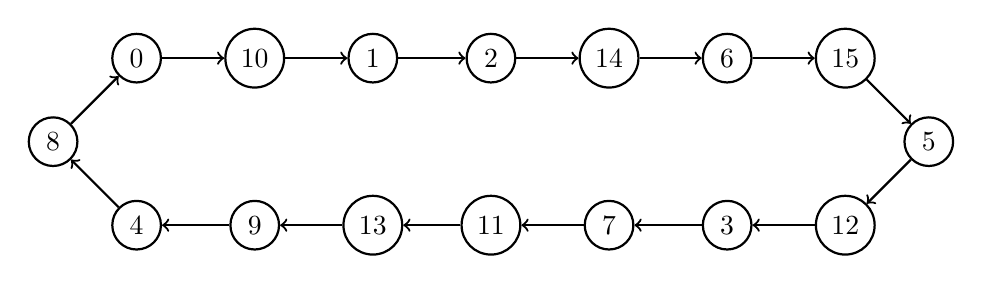
\begin{tikzpicture}[node distance={15mm}, thick, main/.style = {draw, circle}] 
    \node[main] (0) {$0$};
    \node[main] (10) [right of = 0] {$10$};
    \node[main] (1) [right of = 10] {$1$};
    \node[main] (2) [right of = 1] {$2$};
    \node[main] (14) [right of = 2] {$14$};
    \node[main] (6) [right of = 14] {$6$};
    \node[main] (15) [right of = 6] {$15$};
    \node[main] (5) [below right of = 15] {$5$};
    \node[main] (12) [below left of = 5] {$12$};
    \node[main] (3) [left of = 12] {$3$};
    \node[main] (7) [left of = 3] {$7$};
    \node[main] (11) [left of = 7] {$11$};
    \node[main] (13) [left of = 11] {$13$};
    \node[main] (9) [left of = 13] {$9$};
    \node[main] (4) [left of = 9] {$4$};
    \node[main] (8) [above left of = 4] {$8$};
    
    \draw[->] (0) -- (10);
    \draw[->] (10) -- (1);
    \draw[->] (1) -- (2);
    \draw[->] (2) -- (14);
    \draw[->] (14) -- (6);
    \draw[->] (6) -- (15);
    \draw[->] (15) -- (5);
    \draw[->] (5) -- (12);
    \draw[->] (12) -- (3);
    \draw[->] (3) -- (7);
    \draw[->] (7) -- (11);
    \draw[->] (11) -- (13);
    \draw[->] (13) -- (9);
    \draw[->] (9) -- (4);
    \draw[->] (4) -- (8);
    \draw[->] (8) -- (0);
  \end{tikzpicture} 
\end{center}
The code tells us that the traversal terminates when it reaches the node $15$. If all of the nodes are not visited, the bomb will explode, so we need to find a starting point such that it will visit every nodes. Fortunately, this is trivial, as we just need to look at the graph, which is the node $5$. So our first number should be $5$. Reset the bomb and type in ``5 6'' will pass this loop. Let's focus on the last lines
{\renewcommand\fcolorbox[4][]{\textcolor{cyan}{\strut#4}}
\begin{minted}[frame=single,framesep=10pt]{gas}
  0x00000000004010fa <+92>:    cmp    %ecx,0x8(%rsp)
  0x00000000004010fe <+96>:    je     0x401105 <phase_5+103>
  0x0000000000401100 <+98>:    callq  0x401451 <explode_bomb>
  0x0000000000401105 <+103>:   add    $0x18,%rsp
  0x0000000000401109 <+107>:   retq
\end{minted}
}\noindent
From the code above, we know that \verb+%ecx+ is the sum of the nodes that we passed through, let's inspect \verb+0x8(%rsp)+, and \verb+%ecx+
{\renewcommand\fcolorbox[4][]{\textcolor{cyan}{\strut#4}}
\begin{minted}[frame=single,framesep=10pt]{bash}
  (gdb) x 0x8+$rsp
  0x7fffffffe228: 6 # our second input
  (gdb) print $ecx
  $1 = 115
\end{minted}
}\noindent
Therefore, we obtain the correct input for this phase is ``5 115''. Resetting the bomb and type in ``5 115'', we have successfully defused the bomb.
{\renewcommand\fcolorbox[4][]{\textcolor{cyan}{\strut#4}}
\begin{minted}[frame=single,framesep=10pt]{bash}
  [edusc03-052@cheetah022 bomb52]$ ./bomb input.txt
  Welcome to my fiendish little bomb. You have 6 phases with
  which to blow yourself up. Have a nice day!
  Phase 1 defused. How about the next one?
  That's number 2.  Keep going!
  Halfway there!
  So you got that one.  Try this one.
  5 115
  Good work!  On to the next...
\end{minted}
}\noindent
\newpage